\section{Heavy Lift Drone with Infrared Camera}
\label{section:ir_drone}

\begin{figure}
    \centering
    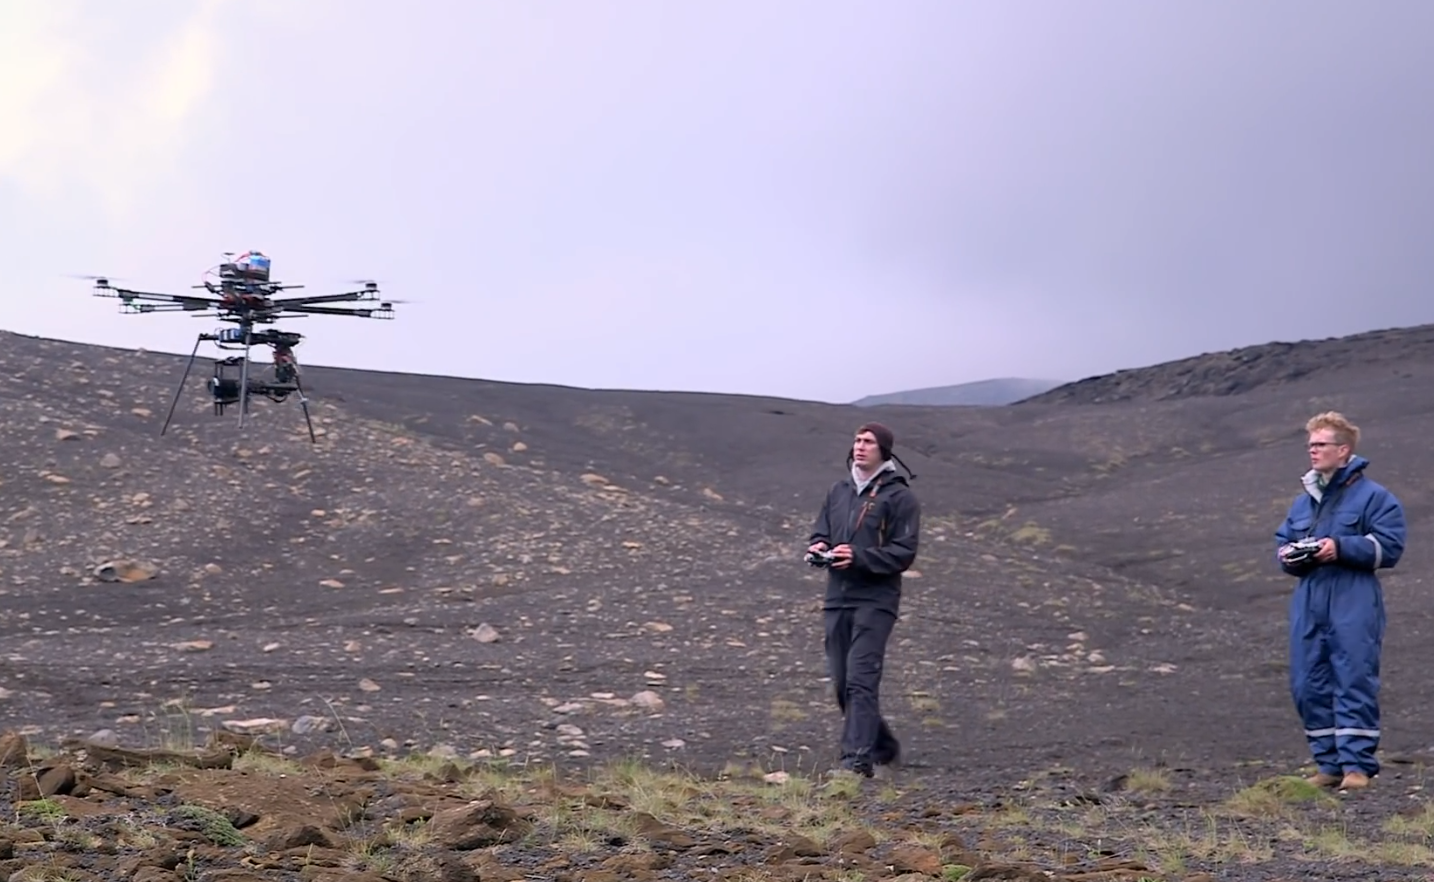
\includegraphics[width=0.75\textwidth]{ir_drone_in_flight}
    \caption{The IR drone in flight with Joshua (left) operating the drone and Baldur (right) operating the gimbal.}
    \label{figure:ir_drone_in_flight}
\end{figure}

Drone-based remote sensing is a new and powerful tool in many fields, including geology.
To this end, Geologist Christopher Hamilton brought a heavy lift drone to Iceland
with the plan of collecting infrared video at active lava sites.
The drone is theoretically capable of lifting itself with an extra load of 25 kg.
This high weight capacity is necessary to lift multiple large batteries,
a large gimbal,
and an infrared camera (FLIR).
The drone before flight can be seen in Figure~\ref{figure:ir_drone_office}.
Along with Baldur, I assembled and tested the drone, making modifications to accomplish the goal of obtaining
aerial IR footage of the lava field in Geldingadalur.

The drone uses a WuKong (DJI) industrial flight controller,
6 2-horsepower motors,
a 22.2 V, 22000 mAh LiPo battery,
and has a diameter of more than a meter.
It sits on a gimbal with the mounted IR camera.
The gimbal uses a 14.8 V battery to control the orientation of the camera,
and receives RC signals from a secondary, dedicated receiver.
(One operator controls the drone while the other controls the gimbal.)
The camera does not have stringent power requirements,
but in this setup the only option for powering it was to provide
a 48 V PoE (Power over Ethernet) source.
A Raspberry Pi 3 connects to the camera over ethernet and records the streamed
video to a file, using a special version of GStreamer developed for the FLIR.

\begin{figure}
    \centering
    \includegraphics[width=0.75\textwidth]{ir_drone_office}
    \caption{The assembled drone before flight.}
    \label{figure:ir_drone_office}
\end{figure}

Due to time constraints (about 48 hours from receipt of the gimbal
to flying over the lava field),
much of the drone has been quickly improvised.
Many of these things must be rectified in the near future for further testing.
For example, the mounting plate between the gimbal and the drone
is completely inadequate (too flexible, not enough points of contact, etc.),
and must be replaced with a more solid/purpose-made mounting plate.
The 48 V requirement of the camera required an additional 3 4S battery packs
wired in series and injected into the ethernet,
and this can be replaced with a transformer that can generate 48 V
from the same 14 V power source that the gimbal uses.
The IR video is not streamed to the operators during flight,
so the operators must guess what the camera is seeing, and attempt to obtain good footage.

Still, even with all these disadvantages, the drone flew successfully two times
over the lava field at Geldingadalur and obtained aerial IR footage of the lava,
as can be seen in Figures \ref{figure:ir_drone_in_flight} and \ref{figure:ir_drone_ir_still}.
Additionally, the BBC program documenting the event\footnote{BBC program documenting the drone flight: \url{https://www.youtube.com/watch?v=6SIgFPhhRPE&t=1190s}}, and the raw IR footage\footnote{\url{https://vimeo.com/580302507}} can be found online.

\begin{figure}
    \centering
    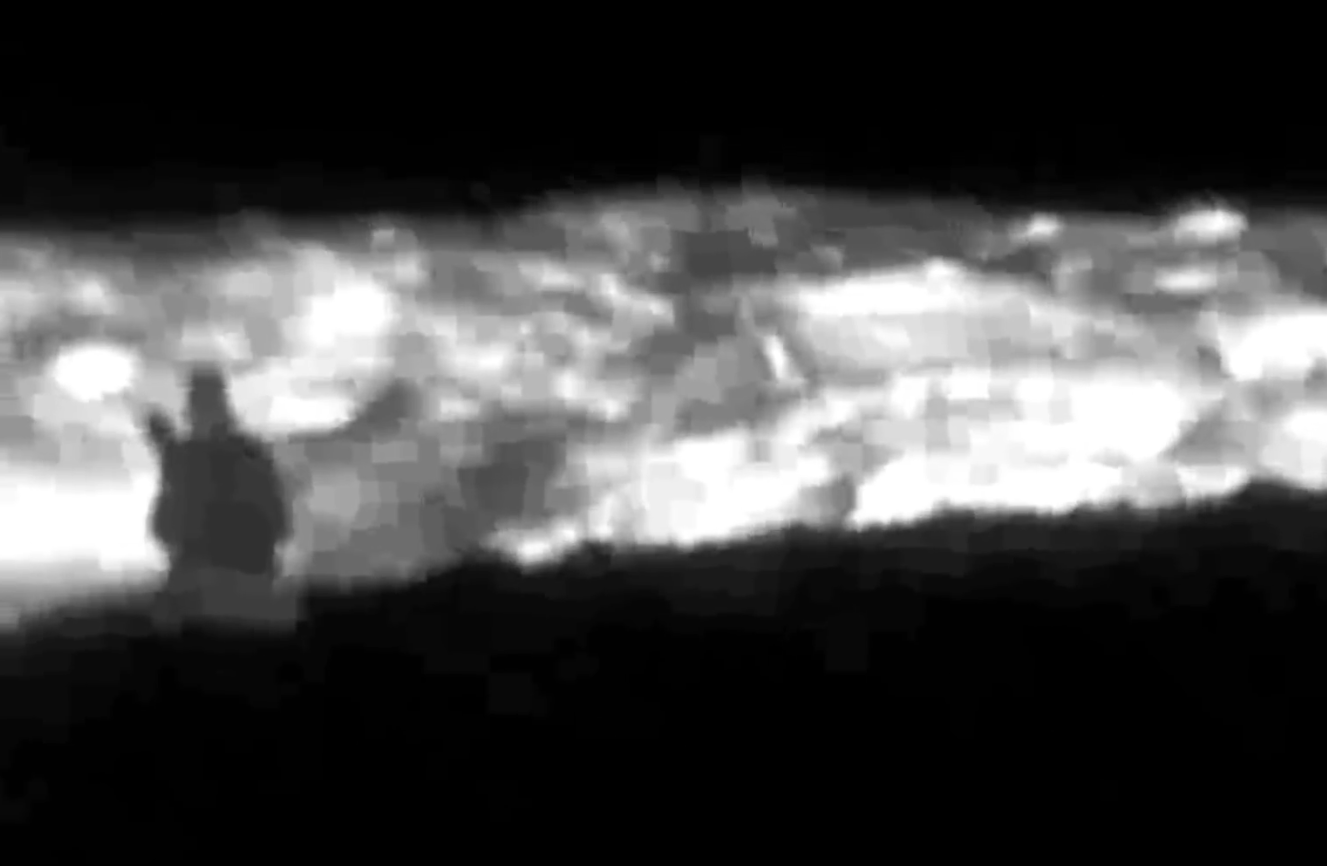
\includegraphics[width=0.75\textwidth]{ir_drone_ir_stillframe}
    \caption{An example still picture from the IR footage of the drone.}
    \label{figure:ir_drone_ir_still}
\end{figure}